\documentclass[]{article}

%=================================
% Fonts, endocing
%=================================
\usepackage[utf8]{inputenc}
\usepackage{fouriernc}

%=================================
% Misc
%=================================
%\usepackage{pgffor}
\usepackage{currfile}



%=================================
% Figures
%=================================
\usepackage{graphicx}
\usepackage{tikzscale}


%=================================
% Graphics
%=================================
\usepackage{pgf}
\usepackage{tikz}
\usepackage{pgfplots}
\usepgfplotslibrary{groupplots,dateplot}
\usetikzlibrary{patterns,shapes.arrows}
\pgfplotsset{compat=newest}



\begin{document}
    \section{Figures}
    Including the following line in your preamble

    \begin{lstlisting}
    \DeclareGraphicsExtensions{.png, .jpg, .pdf, .tikz, .tex}
    \end{lstlisting}

    you tell tex to check for graphics in that order. In other words, 
    by not supplying an extension to  \lstinline|\includegraphics{./figname}|, tex will automatically choose .png before .pdf or .tikz.
    You can later change the priority order if you want. 



    \begin{figure}[htbp]
        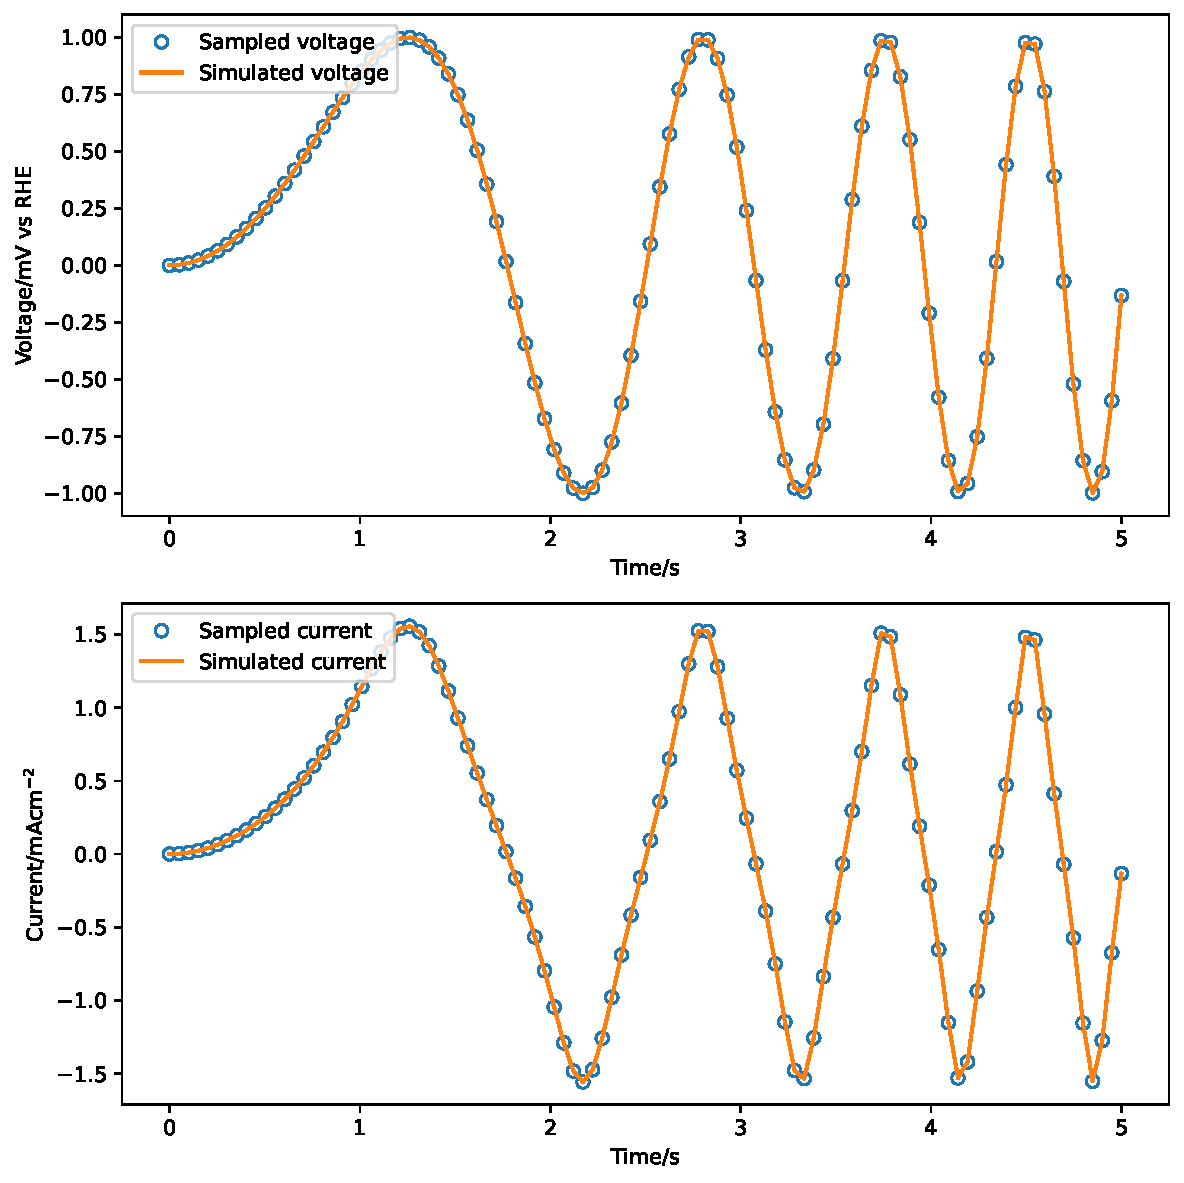
\includegraphics[width=0.7\textwidth]{./figs/example_1}
        \caption{Figure example included withour file extension}
        \label{figures:fig:example:1}
    \end{figure}

    You can still specify an extension if you like. This was done in \cref{figures:fig:example:2}. 
    Notice the difference between \cref{figures:fig:example:2:a,figures:fig:example:2:b} and \cref{figures:fig:example:2:c}.
    The former have simply been scaled to width, while the latter has been generatex from .tikz code.

    \begin{figure}
        \begin{subfigure}[t]{0.32\textwidth}
        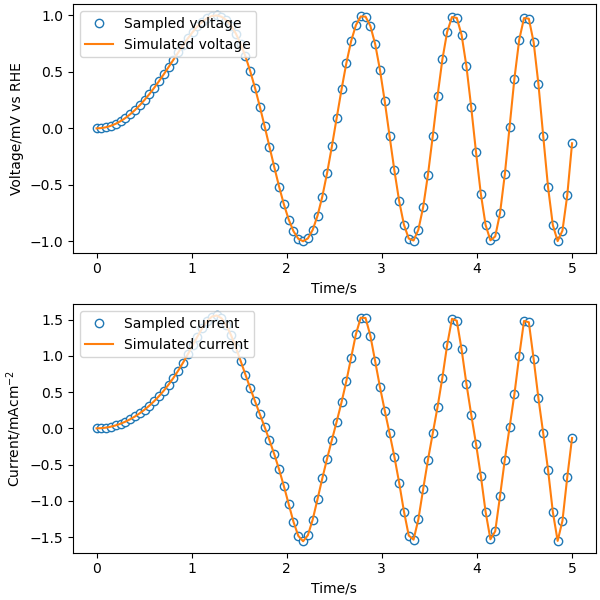
\includegraphics[width=\linewidth]{./figs/example_1.png}
        \caption{.png}
        \label{figures:fig:exmaple:2:a}
        \end{subfigure}
        %
        \begin{subfigure}[t]{0.32\textwidth}
        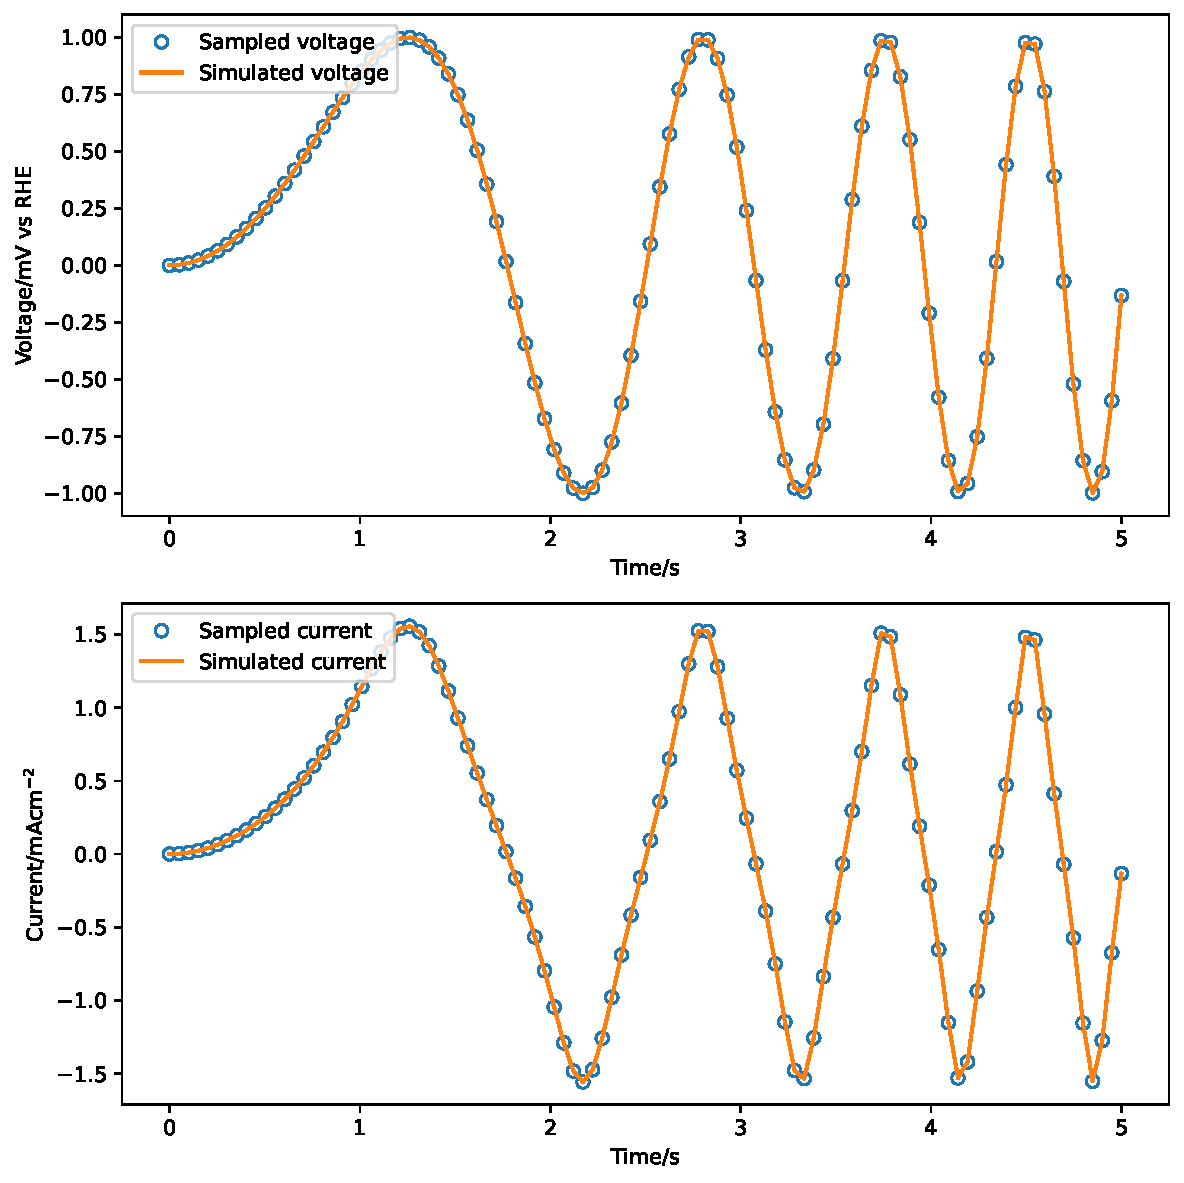
\includegraphics[width=\linewidth]{./figs/example_1.pdf}
        \caption{.pdf}
        \label{figures:fig:exmaple:2:b}
        \end{subfigure}
        %
        \begin{subfigure}[t]{0.32\textwidth}
        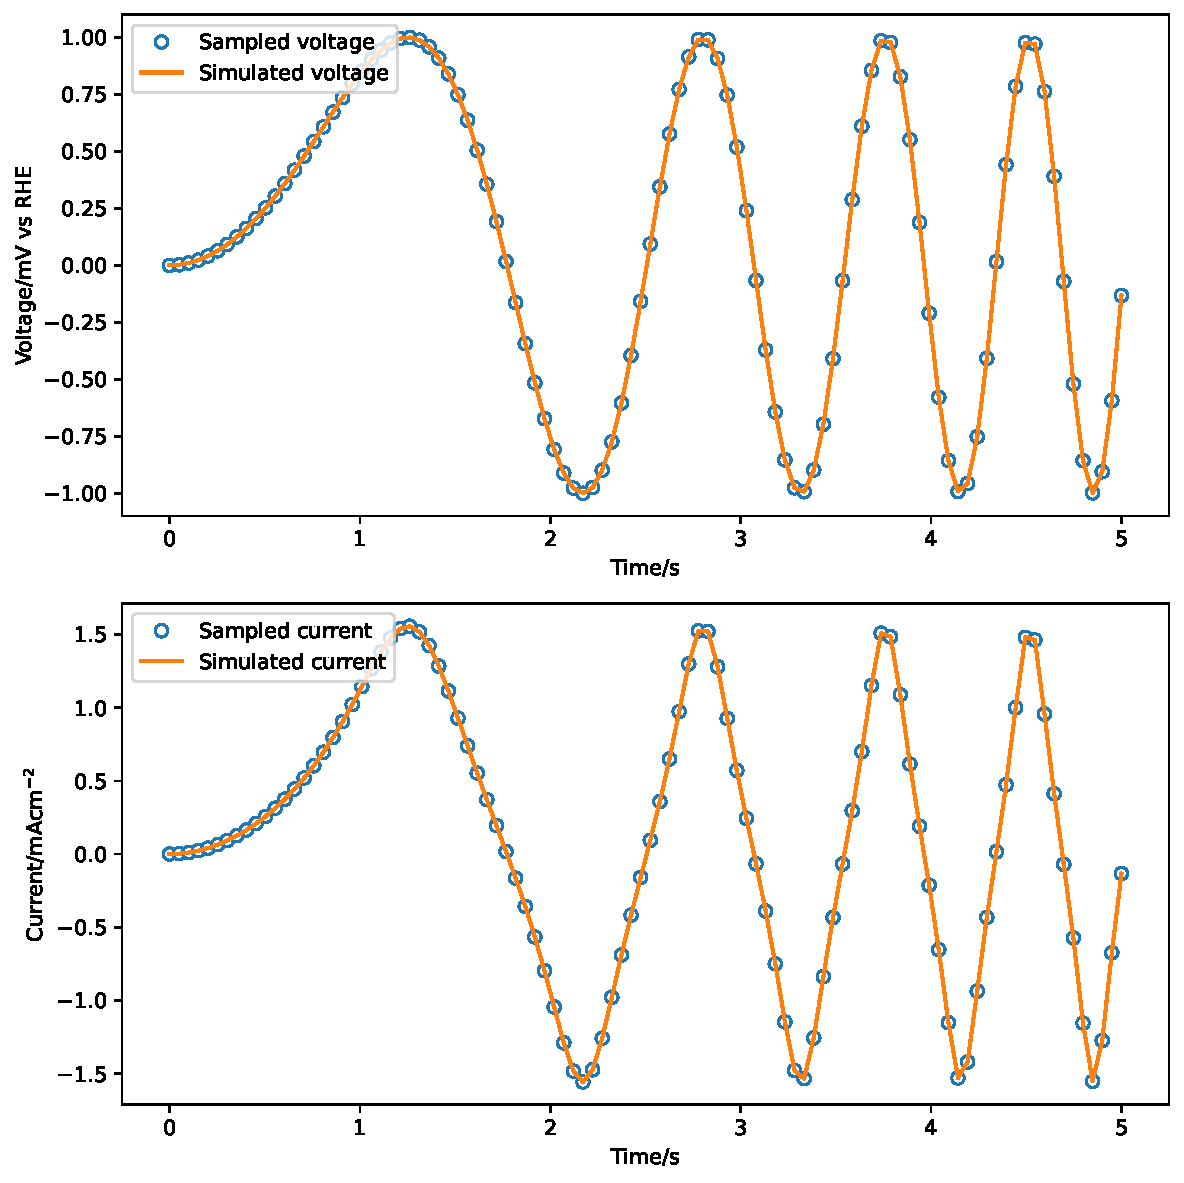
\includegraphics[width=\linewidth]{./figs/example_1.tikz}
        \caption{.tikz}
        \label{figures:fig:exmaple:2:c}
        \end{subfigure}     
        \caption{Figures included by specifying file extension.}   
        \label{figures:fig:example:2}
    \end{figure}


\end{document}